\section{Results}
\label{sec:results}

\subsection{Baseline Estimates}

Table \ref{tab:main} reports the baseline DiD estimates. Panel A compares high-TDDI firms with the rest of the sample. Column (1) shows that high-TDDI firms experience a 0.0917 relative decline in log Tobin's Q after the shock, with a standard error of 0.0343; the estimate is significant at the 1\% level. Relative to the sample mean, this is a 9.2\% valuation discount. Column (2) shows that the level of Tobin's Q declines by 0.3596 (standard error 0.1244). Column (3) shows that gross margin declines by 2.45 percentage points (standard error 1.10), significant at the 5\% level. Columns (4) and (5) show that ROA and the selling-expense ratio change by 0.0004 and $-0.0093$, respectively, and neither effect is significant. The period-expense ratio is also insignificant ($-0.0071$, standard error 0.0091; not tabulated).

Panel B reports the continuous specification. A one-standard-deviation increase in TDDI is associated with a 0.0395 decline in log Tobin's Q (standard error 0.0171), a 0.1700 decline in Tobin's Q (standard error 0.0657), and a 1.24 percentage-point decline in gross margin (standard error 0.53), all significant at the 5\% level. ROA and selling-expense ratios remain insignificant. The continuous and binary specifications point in the same direction and are of comparable magnitude: the binary coefficient is approximately the continuous coefficient scaled by the average TDDI difference between the high group and the rest.

The economic magnitude is substantial. The high-TDDI group had a combined equity market value of RMB 1.72 trillion in 2021Q1. Applying the 9.2\% discount implies a market-value loss of about RMB 203.7 billion (Section 10). This estimate covers only the third-party data channel; it excludes first-party data, algorithms, brands, and network effects. It is therefore a lower bound on the value of the firms' data-related assets, not an estimate of their total data value.

\begin{table}[htbp]
\centering
\small
\setlength{\tabcolsep}{4pt}
\caption{Baseline difference-in-differences estimates.}
\label{tab:main}
\begin{threeparttable}
\begin{tabular}{lccccc}
\toprule
(1) Log Tobin's Q & (2) Tobin's Q & (3) Gross margin & (4) ROA & (5) Selling-expense ratio \\
\midrule
\multicolumn{6}{l}{Panel A: High-TDDI firms (top third)} \\
High TDDI $\times$ Post & -0.0917*** & -0.3596*** & -0.0245** & 0.0004 & -0.0093 \\
 & (0.0343) & (0.1244) & (0.0110) & (0.0023) & (0.0077) \\
\midrule
\multicolumn{6}{l}{Panel B: Continuous TDDI (one-standard-deviation increase)} \\
TDDI $\times$ Post & -0.0395** & -0.1700*** & -0.0124** & -0.0002 & -0.0018 \\
 & (0.0171) & (0.0657) & (0.0053) & (0.0013) & (0.0031) \\
\midrule
Controls & Yes & Yes & Yes & Yes & Yes \\
Firm FE & Yes & Yes & Yes & Yes & Yes \\
Industry $\times$ Quarter FE & Yes & Yes & Yes & Yes & Yes \\
Observations & 6,900 & 6,900 & 6,897 & 6,900 & 6,866 \\
$R^2$ & 0.221 & 0.158 & 0.019 & 0.027 & 0.001 \\
\bottomrule
\end{tabular}
\begin{tablenotes}[flushleft]
\footnotesize
\item Notes: Standard errors clustered by firm are in parentheses. ***, **, and * denote significance at the 1\%, 5\%, and 10\% levels. Post equals one for 2021Q3 and later. High TDDI indicates the top third of the TDDI distribution; the comparison group is the rest of the sample. Controls include lagged firm size, leverage, and the cash ratio. The TDDI is standardized in Panel B.
\end{tablenotes}
\end{threeparttable}
\end{table}


\begin{figure}[htbp]
\centering
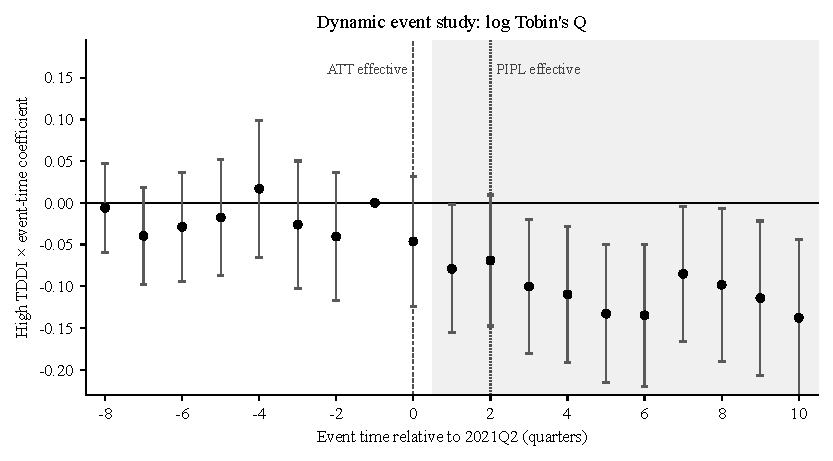
\includegraphics[width=0.95\textwidth]{fig3_event_study.pdf}
\caption{Dynamic event study for log Tobin's Q. Points are coefficients on the interaction between the high-TDDI indicator and event-time dummies; vertical bars are 95\% confidence intervals. The omitted period is 2021Q1 ($k=-1$), shown as a hollow point. Regressions include firm fixed effects, industry-by-quarter fixed effects, and controls. The joint test on the leads yields $p=0.079$. The shaded area is the post-shock period.}
\label{fig:event}
\end{figure}

\subsection{Dynamic Effects}

Figure \ref{fig:event} shows the event-study estimates. The lead coefficients from 2019 to 2020 fluctuate around zero and are individually insignificant. The 2021Q2 coefficient is $-0.046$ and insignificant; the 2021Q3 coefficient is $-0.079$ and significant at the 5\% level. The effect then grows steadily: $-0.100$ in 2022Q1, $-0.133$ in 2022Q3, and $-0.138$ in 2023Q4. The joint test on the leads yields $p=0.079$, which is at the margin of conventional significance. The largest negative lead is about $-0.04$, roughly half the size of the post-shock effect. We therefore interpret the post-shock decline as a break rather than a continuation of a pre-existing trend, and we report placebo and robustness tests in Section 9.4.

The gradual path is consistent with the institutional setting. ATT took effect at the end of Q2 2021, and PIPL took effect in November 2021. Firms needed time to adjust their data collection, advertising technology, and compliance processes. Investors also needed time to reassess the long-run rents from third-party data. The event-study pattern—small and insignificant at the onset, larger and more precise after several quarters—matches this adjustment process.

\subsection{Dose-Response}

Figure \ref{fig:dose} reports the quintile dose-response. Relative to the lowest quintile, the second quintile's coefficient is 0.010 and insignificant, the third is $-0.037$, the fourth is $-0.090$, and the fifth is $-0.090$. The decline occurs mainly between the third and fourth quintiles and then flattens. The highest quintile is significant at the 10\% level, and the top-third versus bottom-third comparison is significant at the 5\% level (Table \ref{tab:hetero}). The pattern indicates a nonlinear dose-response: valuation losses rise sharply once TDDI exceeds the middle of the distribution, and then saturate at the top.

The saturation is economically plausible. Firms in the top quintile are already highly dependent on third-party data; further increases in the text-based index do not necessarily imply proportionally larger exposure. The binary top-third specification captures the economically relevant contrast without imposing a linear relationship across the entire distribution.

\begin{figure}[htbp]
\centering
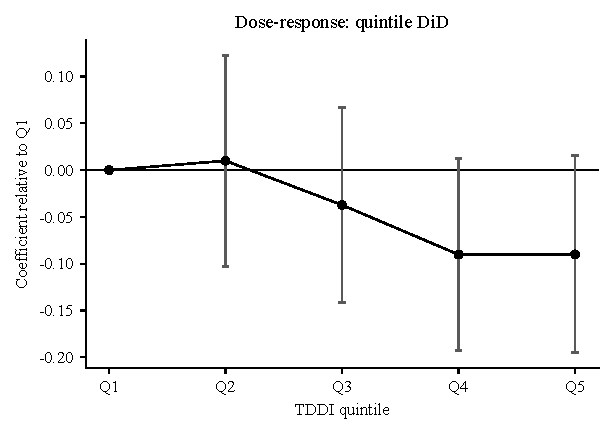
\includegraphics[width=0.72\textwidth]{fig4_dose_response.pdf}
\caption{Dose-response by TDDI quintile. Points are coefficients on the interaction between the quintile indicator and the post-shock dummy; the first quintile is the omitted reference group. Vertical bars are 95\% confidence intervals. Regressions include firm fixed effects, industry-by-quarter fixed effects, and controls.}
\label{fig:dose}
\end{figure}

\subsection{Placebo Tests}

We assign pseudo-shock dates in 2019Q3 and 2020Q3 and restrict the sample to the pre-2021 period. The coefficients on high TDDI interacted with the pseudo-shock are $-0.032$ (standard error 0.033) and $-0.032$ (standard error 0.032), respectively, and neither is significant. Replacing the TDDI with the generic digitalization index yields a coefficient of $-0.021$ (standard error 0.019), also insignificant. In a horse race that includes both high TDDI and high generic digitalization, the TDDI coefficient is $-0.075$ (standard error 0.036) and the generic digitalization coefficient is $-0.040$ (standard error 0.035), with only the former significant. The results are therefore not driven by a pre-existing trend or by a generic digitalization narrative.
